%!TEX root = presentazionelancia.tex
\section{Selección}

\begin{frame}[c] 
\centering
\huge \textbf{Estructuras de selección}
\end{frame}


\begin{frame}[c]\frametitle{Estructuras de selección}
%\centering
%\includegraphics[width=\textwidth]{figs/table3.pdf} 
    Las estructuras de selección se utilizan cuando en el desarrollo de la solución de un problema se debe \textbf{tomar una decisión}, para establecer un proceso o señalar un camino alternativo a seguir.\\
    \vspace*{2mm}
    Esta toma de decisión se basa en la evaluación de una o más condiciones que señalarán, como alternativa o consecuencia, la \textbf{rama} a seguir.\\
    \vspace*{35mm}
    \tiny Battistutti, O. C. (2005). Metodología de la programación: Algoritmos, diagramas de flujo y programas (3rd ed.). México, D.F.: Alfaomega.
\end{frame}


\begin{frame}[c] \frametitle{Estructuras de selección}
Las estructuras algorítmicas selectivas que se utilizan para la toma de decisiones lógicas las podemos clasificar de la siguiente forma:
\begin{itemize}
    \item \textbf{SI - ENTONCES:} selección sencilla.
    \item \textbf{SI - ENTONCES / SINO:} selección doble.
    \item \textbf{SI MULTIPLE:} selección múltiple.
\end{itemize}
\vspace*{40mm}
\tiny Deitel, H. M., & Deitel, P. J. (1995). Cómo programar en C/C (4th ed.). México: Prentice Hall.
\end{frame}


\begin{frame}[c] \frametitle{Selección sencilla}
La estructura selectiva \textbf{SI - ENTONCES} permite que el flujo de datos siga por un camino específico si se cumple una condición o conjunto de condiciones. \\
\vspace*{2mm}
Si al evaluar la condición (o condiciones) el resultado es verdadero, entonces se ejecutan un conjunto de operaciones. \\
\vspace*{2mm}
Luego, se continúa con la secuencia normal del flujo.
\vspace*{35mm}
\tiny Battistutti, O. C. (2005). Metodología de la programación: Algoritmos, diagramas de flujo y programas (3rd ed.). México, D.F.: Alfaomega.
\end{frame}


\begin{frame}[c] \frametitle{Diagrama de flujo de la selección sencilla}
\begin{center}
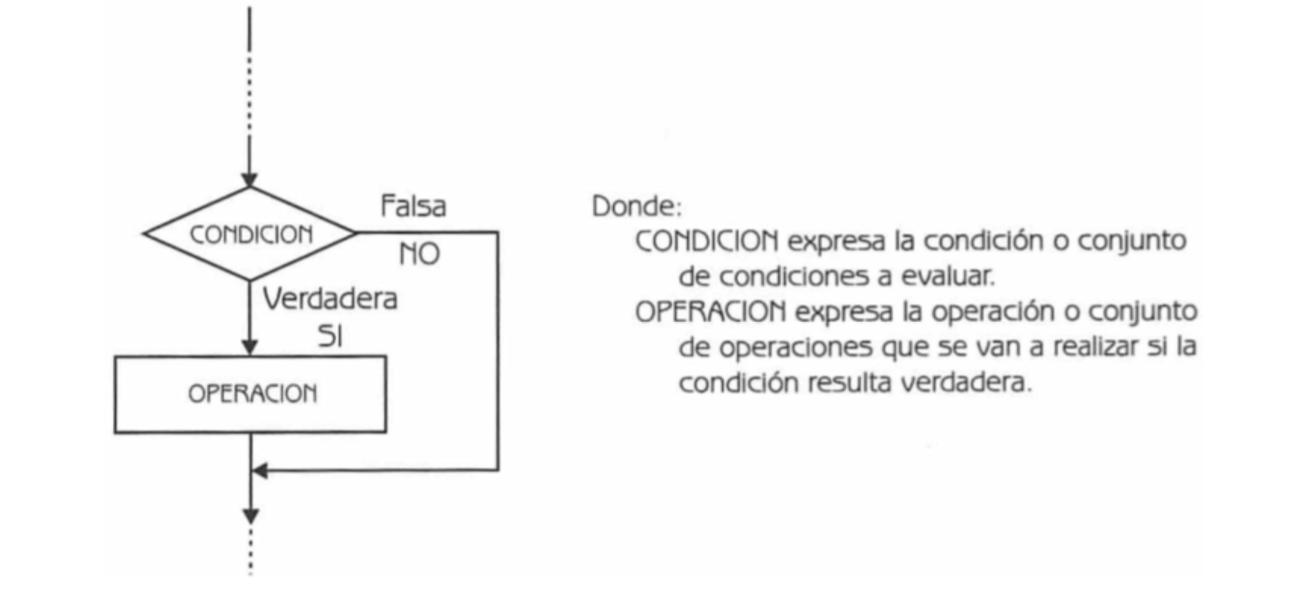
\includegraphics[width=\textwidth]{figs/SeleccionSencillaDF.png}
\end{center}
\vspace*{10mm}
\tiny Battistutti, O. C. (2005). Metodología de la programación: Algoritmos, diagramas de flujo y programas (3rd ed.). México, D.F.: Alfaomega.
\end{frame}


\begin{frame}[fragile, c] \frametitle{Estructura de la selección sencilla}
\begin{lstlisting}
...
if(CONDICION)
{
    OPERACION
}
...
\end{lstlisting}
\vspace*{35mm}
%\tiny Aguilar, L. J., & Martínez, I. Z. (2010). Programación en C: Metodología, algoritmos y estructura de datos. Madrid: McGraw-Hill.
\end{frame}






